% !TEX root = thesis.tex

\section{Experimental Setup}
\label{sec:exp}
\subsection{CERN}
The European Organization for Nuclear Research (CERN), established in 1954, operates the largest particle physics laboratory in the world. In 2019 CERN consists of 22 member states. Additionally CERN has contacts with a number of associate member states and various individual institutions. The laboratory, also referred to as CERN, itself is located near Geneva at the border of France and Switzerland employs about 2500 people. Additionally some 12000 visiting scientists from over 600 institutions in over 70 countries come to CERN for their research. 

\begin{figure}[htb]
\centering
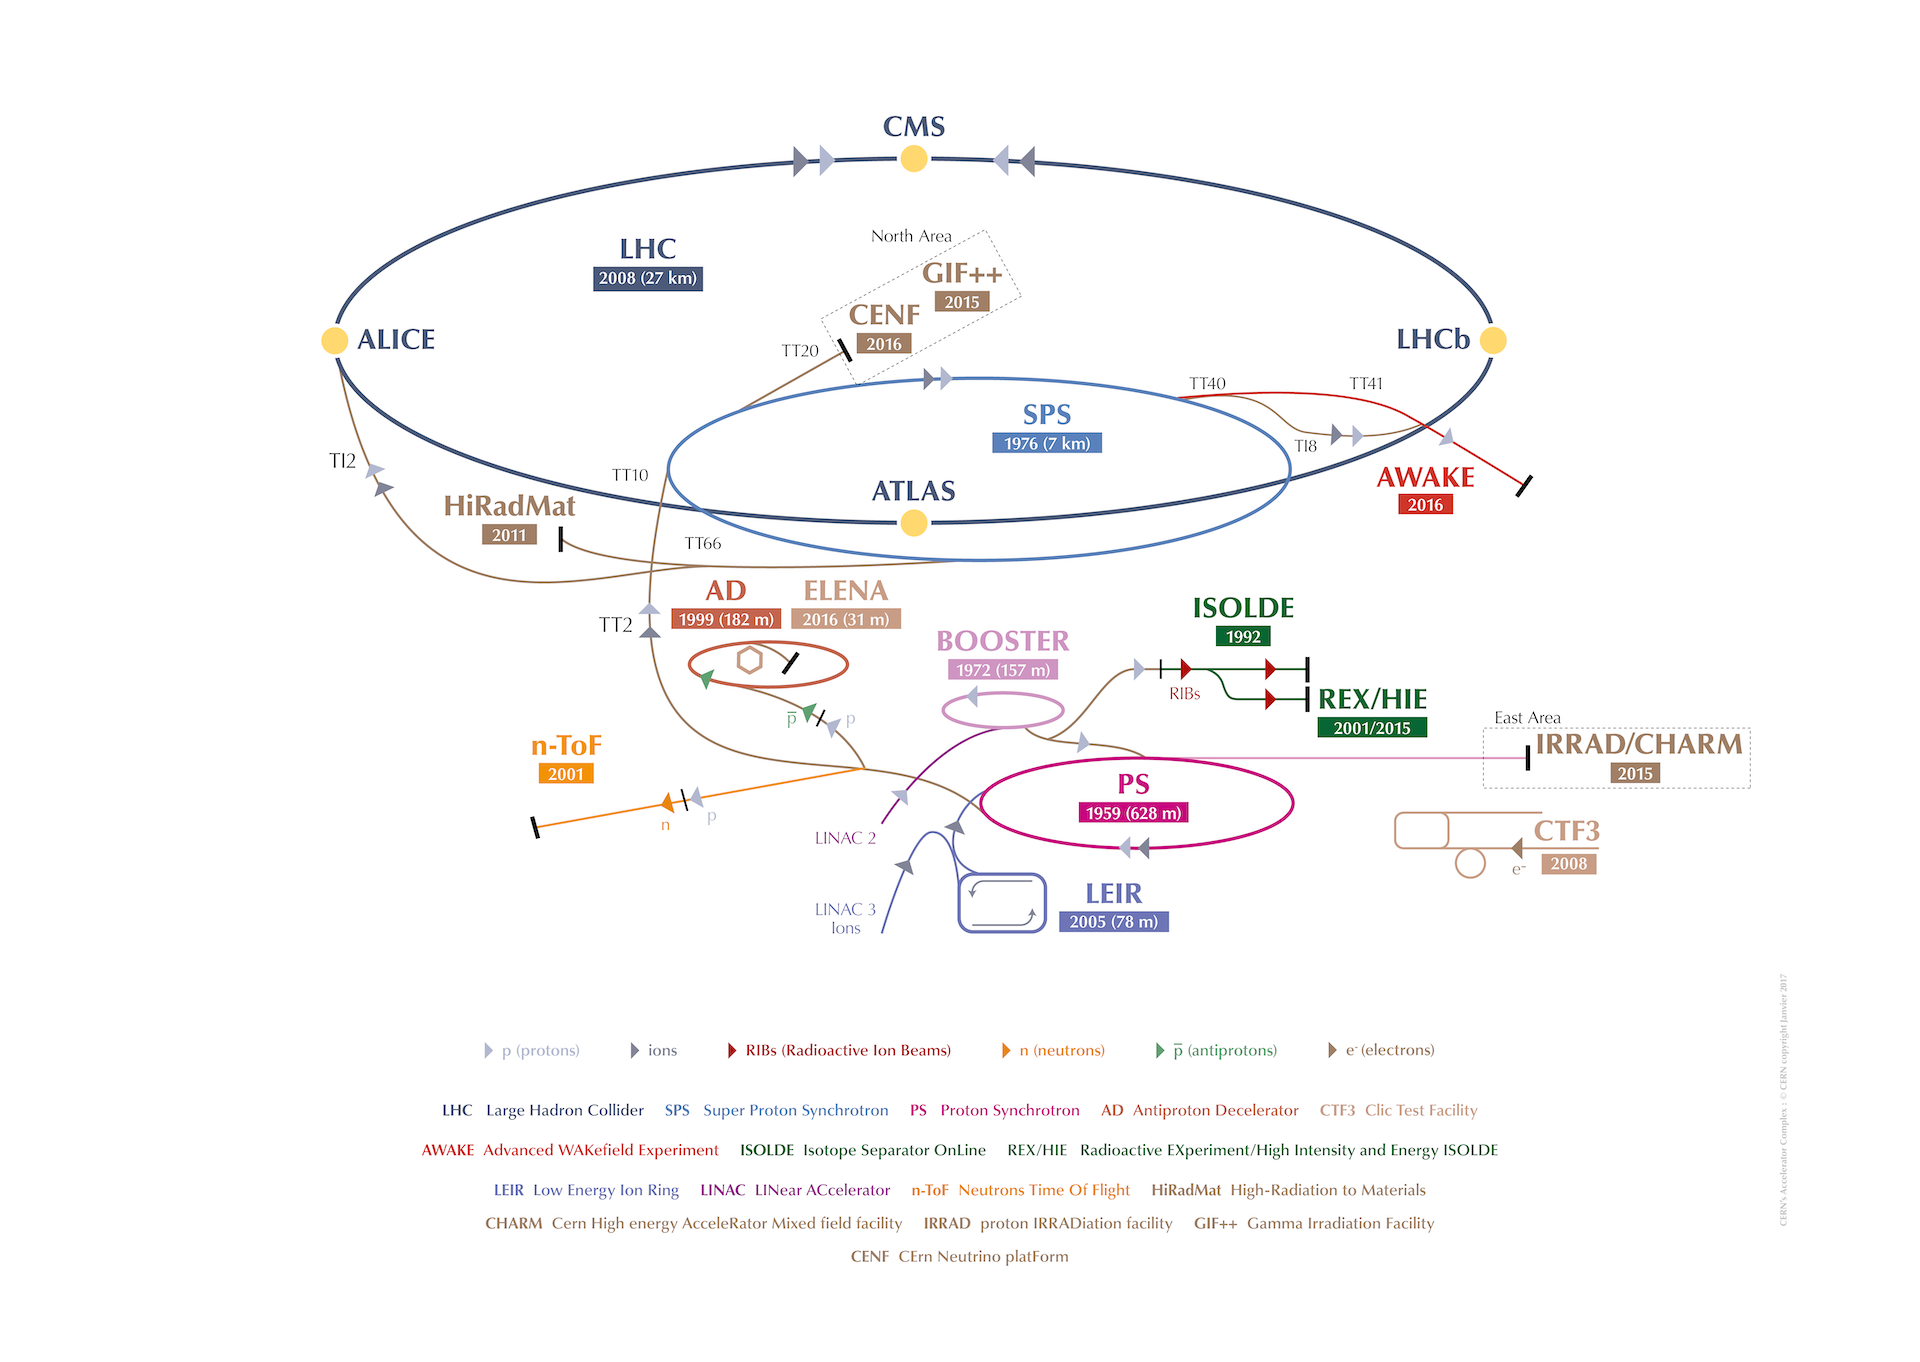
\includegraphics[width=0.9\textwidth]{pics/CernCollidersSmall}
\caption[CERN collider complex]{ A schematic view of the accelerator complex at CERN. Before particles can be injected into the LHC they require a series of accelerators with increasing size. Until 2018 protons started their journey in LINAC2 (Linear Accelerator) and continue through the Booster, Proton Synchrotron (PS) and Super Proton Synchrotron (SPS). Between 2019 and 2020 LINAC2 will be replaced by LINAC4~\cite{CernComplex}}
\label{fig:CernComplex}
\end{figure}

The laboratory includes a series of accelerators, which are used to accelerate the particle beams used. A schematic view of the complex as of 2019 is shown in Figure~\ref{fig:CernComplex}. In the framework of this thesis the most important component is the Large Hadron Collider (LHC), the largest collider at CERN. LHC will be discussed in more detail in Sec.~\ref{sec:lhc}. Other accelerators in the series are used to inject the particle beams into LHC, but they are also used in itself for various experimental studies. 

The second largest accelerator is the super proton synchrotron (SPS). It is the final step before the particle beam is injected into LHC. Commissioned in 1976, it was the largest accelerator at CERN until the the Large Electron-Positron Collider (LEP) was finished in 1989. Originally it was used as a proton-antiproton collider and as such provided the data for the UA1 and UA2 experiments, which resulted in the discovery of the W and Z bosons~\cite{Watkins:1986va}. At the moment there are several fixed target experiments utilising the beam from the SPS. These study the structure (COMPASS) and properties (NA61/SHINE) of hadrons, rare decays of kaons (NA62) and radiation processes in strong electromagnetic fields (NA63). Additionally the AWAKE and UA9 experiments are used for accelerator research and development. 

The third largest accelerator in CERN is the proton synchrotron (PS). Capable of accelerating beams up to an energy of \unit[25]{\gev} PS provides the beam to SPS. Additionally PS has experiments for studying strong force (DIRAC), the effect of cosmic rays on cloud formation (CLOUD) and neutron-nucleus interactions (nTOF).

Additionally PS provides the beam to the antiproton decelerator (AD), which uses the beam and a block of metal to produce antiprotons. These are then decelerated in AD into a useful low-energy beam, which is provided to a host of experiments studying the properties of antimatter.

PS gets proton beams from LINAC2 through BOOSTER and ion beams from LINAC3 through LEIR. From BOOSTER beams are also provided to the On-Line Isotope Mass Separator (ISOLDE). ISOLDE directs the beam into thick targets to produce low energy beams of radioactive nuclei. These beams are used to study the properties of even the most exotic of atomic nuclei in a host of experiments.

More information of the various experiments at CERN can be found online from ~\cite{CERNexperiments}.

\subsection{Large Hadron Collider}
\label{sec:lhc}
The Large Hadron Collider (LHC) with its circumference of \unit[26.7]{km} is the largest accelerator at CERN and the largest particle collider ever built. The LHC is designed to accelerate protons up to an energy of \unit[8]{\tev} and lead ions up to \unit[2.76]{\tev} per nucleon~\cite{Bruning:782076}. The design luminosity of the LHC is $ \unit[10^{34}]{cm^{-2}s^{-1}}$. In 2017 it achieved a record peak luminosity of $ \unit[2\cdot10^{34}]{cm^{-2}s^{-1}}$. For lead beams luminosities of up to $ \unit[6\cdot10^{27}]{cm^{-2}s^{-1}}$ were reached in 2018. All this is achieved with a ring consisting of 1232 superconducting dipole magnets that keep particles in orbit. 

The LHC receives beams with energies of \unit[450]{\gev} from the SPS. In the LHC the particles are accelerated through the use of radio-frequency (RF) cavities. Electromagnetic waves become resonant and build up inside the cavity. As they consist of electromagnetic waves, the field in the RF cavity oscillates. Charges passing through the cavity feel the overall force and are pushed forward along the accelerator. Particles must enter the cavity at the correct phase of oscillation to receive a forward push. When timed correctly, the particles will feel zero accelerating voltage when they have exactly the correct energy. Particles with higher energies will be decelerated  and particles with lower energies will be accelerated. This focuses particles in distinct bunches. The RF oscillation frequency at the LHC is 400.8 MHz. Thus  RF "buckets" are separated by 2.5 ns. However only 10 \% are actually filled with particles, so the bunch spacing in the LHC is 25 ns, at a bunch frequency of 40 MHz.

With 7 TeV proton beams the dipole magnets used to bend the beam must produce a magnetic field of 8.33 T. This can be only achieved through making the magnets superconducting, which requires cooling them down with helium to a temperature of 1.9 K. The 1232 dipole magnets make up roughly 2/3 of the LHC circumference. The remaining part is made up of the RF cavities, various sensors and higher multipole magnets used to keep the beam focused. The most notable of these are the 392 quadrupole magnets.

The LHC is divided into octants, where each octant has a distinct function. Octants 2 and 8 are used to inject beam into the LHC from SPS. The 2 beams are crossed in octants 1,2,5 and 8. The main experiments are built around these crossing points. Octants 3 and 7 are used for beam cleansing. This is achieved through collimators that scatter particles with too high momentum or position offsets off from the beam. The RF cavities used for acceleration are located in octant 4 and octant 6 is used for dumping the beam. The beam dump is made up of two iron septum magnets, one for each beam, that will kick the beam away from machine components into an absorber when needed. 


\subsubsection{LHC experiments}
As of 2018 there are four main experiments at the LHC; ALICE, ATLAS, CMS and LHCb and three smaller ones LHCf, TOTEM and MoEDAL. ALICE will be covered in detail in section ~\ref{sec:alice}. 

ATLAS (A Toroidal LHC ApparatuS) and CMS (Compact Muon Solenoid) are the two largest experiments at the LHC. They are both multipurpose experiments designed to be sensitive to many different possible new physics signals, such as extra dimensions and dark matter particles. The biggest discovery made by these so far is the discovery of the Standard Model Higgs boson, which was simultaneously published by the experiments in 2012 ~\cite{Aad:2012tfa, Chatrchyan:2012xdj}.

The LHCb (LHC beauty) experiment ~\cite{Alves:2008zz} is made for studying the bottom (beauty) quark. Main physics goals of the LHCb include the measurement of the parameters of CP violation with decays of hadrons containing the bottom quark. One of the most important results published by LHCb is the first measurement of $B_s^0\rightarrow \mu^+ \mu^-$ decay, which was found to be in line with the Standard Model.

In addition to the four large experiments there are three smaller experiments along the LHC ring. LHCf (LHC forward)~\cite{Adriani:2008zz} is located at interaction point 1 with ATLAS. It aims to simulate cosmic rays by the particles thrown forwards by the collisions in ATLAS.

TOTEM (TOTal Elastic and diffractive cross section Measurement) is located near the CMS experiment at point 5. This allows it to measure particles emerging from CMS with small angles. The main goals is to measure the total, elastic and inelastic cross-sections in pp collisions~\cite{Anelli:2008zza}.

The MoEDAL (Monopole and Exotics Detector At the LHC) experiment~\cite{MoEDAL:2016jlb} is located at the interaction point 8 together with the LHCb experiment. MoEDAL tries to measure signatures of hypothetical particles with magnetic charge, magnetic monopoles.




\subsection{ALICE}
\label{sec:alice}
\begin{figure}[htb]
\documentclass[border=5mm]{standalone}
\usepackage{tikz}
\usetikzlibrary{positioning}
\usetikzlibrary{intersections, calc, fadings}
\begin{document}
\definecolor{primary}{HTML}{0000FF}
\definecolor{secondary}{HTML}{FF8000}
\definecolor{tertiary}{HTML}{00FFFF}


\begin{tikzpicture}
% draw image
\coordinate[] (O);
\coordinate[above =1cm of O,label={right:$y$}] (y);
\coordinate[below left=1cm and 2cm of O, label={below:$x$}] (x);
\coordinate[above left=0.5cm and 4cm of O, label={left:$z$}] (z);

\draw[blue, thick, ->] (O) --  (y);
\draw[blue, thick, ->] (O) -- (x);
\draw[blue, thick, ->] (O) -- (z);

\end{tikzpicture}
\end{document}
\centering
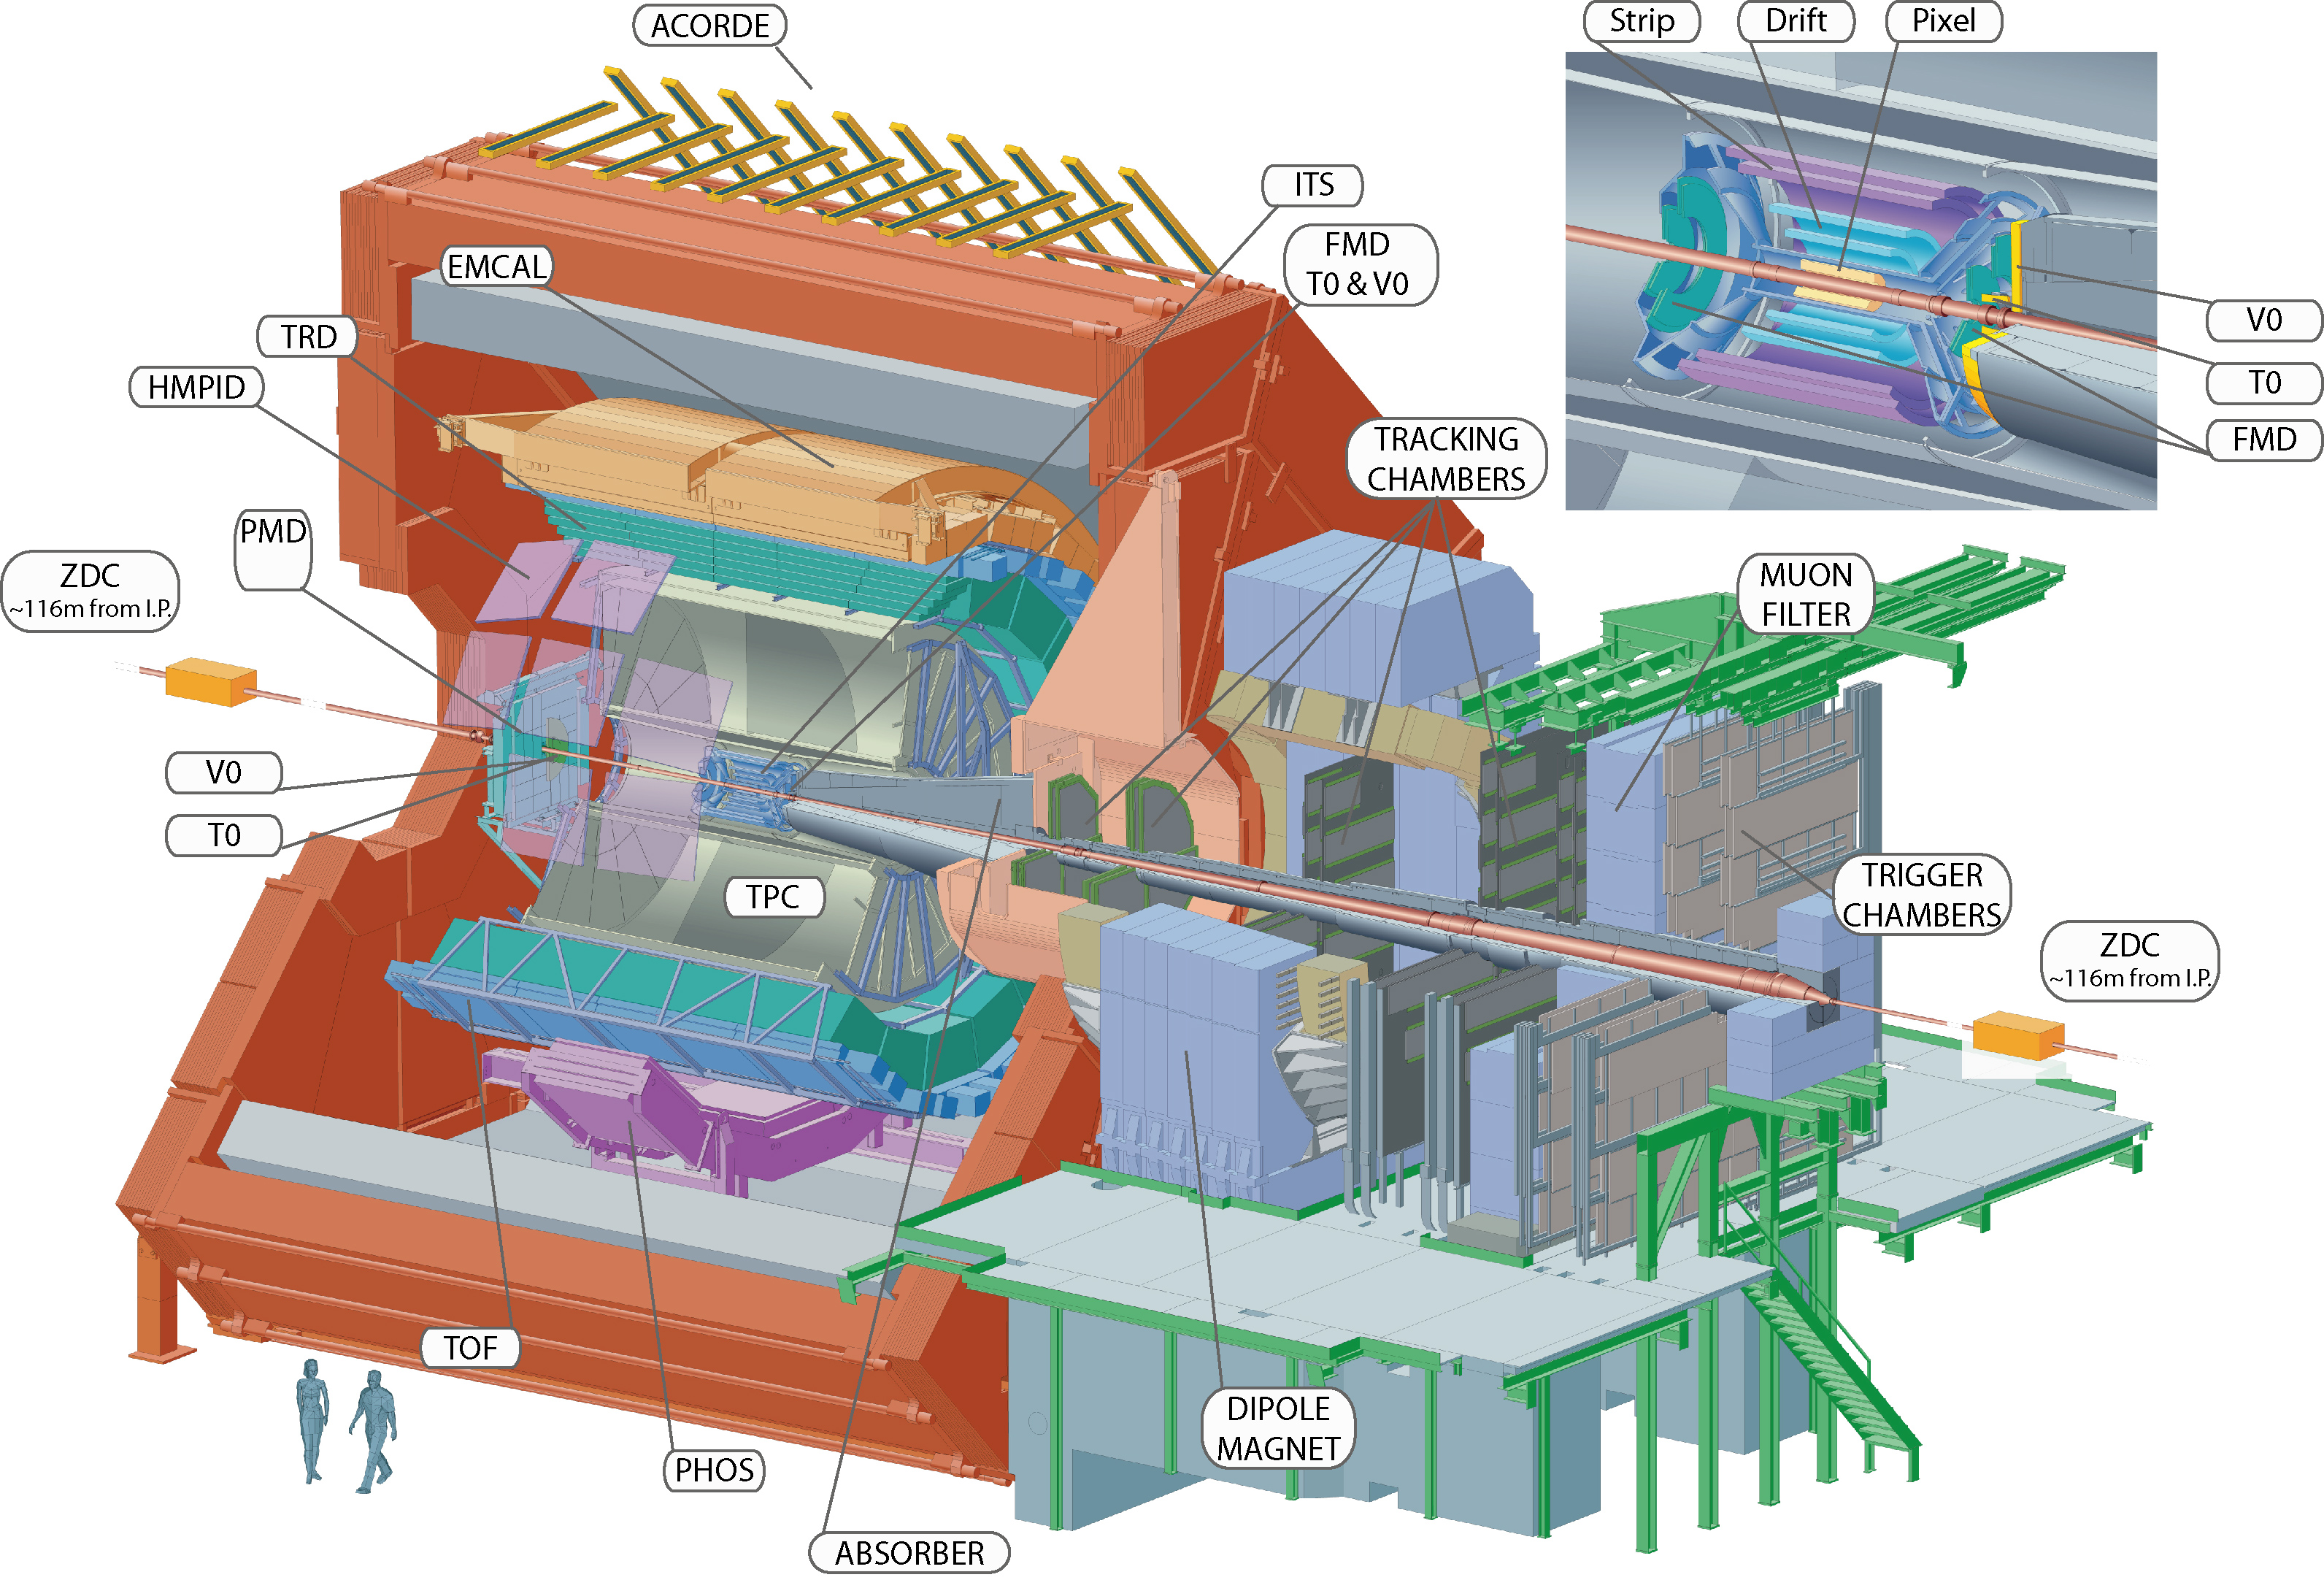
\includegraphics[width=0.95\textwidth]{pics/2012-Aug-02-ALICE_3D_v0_with_Text.jpg}
\caption[ALICE]{Schematic view of the ALICE detector with the definition of coordinates. The positive direction of $z$ is also referred to as the A side and the negative direction as the C side}
\label{fig:alice}
\end{figure}

ALICE (A Large Ion Collider Experiment)~\cite{ALICE} is the dedicated heavy ion experiment at the LHC. ALICE was designed to cope with the expected very high multiplicity environment of heavy ion collisions. The design allows measurement of a large number of low momentum tracks. The different detector subsystems are optimised to provide high momentum resolution and excellent particle identification capabilities over a broad range of momentum.

A schematic view of the ALICE detector in 2018 is presented in Figure ~\ref{fig:alice}. This section will go through the composition of ALICE as it has been during run 2 between 2014 and 2018. The detector will go through significant upgrades during Long Shutdown 2 (LS2) in 2019-2020. 

As in all the major high energy physics experiments the positioning of the detectors follows a layered structure. Closest to the interaction point are the tracking detectors. The main task of these detectors is to locate the position of the primary interaction vertex accurately and to record the tracks of charged particles. To achieve this they need a very good spatial resolution close to the interaction point. Tracking detectors do not significantly alter the tracks of traversing particles. Thus they can be located in the innermost layers.

Calorimeters are designed to stop any particles hitting them and use the absorption to measure the energy of the particles. Thus they must be located behind the tracking detectors. ALICE has two separate calorimeter systems, the electromagnetic calorimeters measure mainly electrons and photons, while the muon detection system measures muons.


\subsubsection{Tracking}
\label{sec:tracking}

\begin{figure}[htb]
\centering
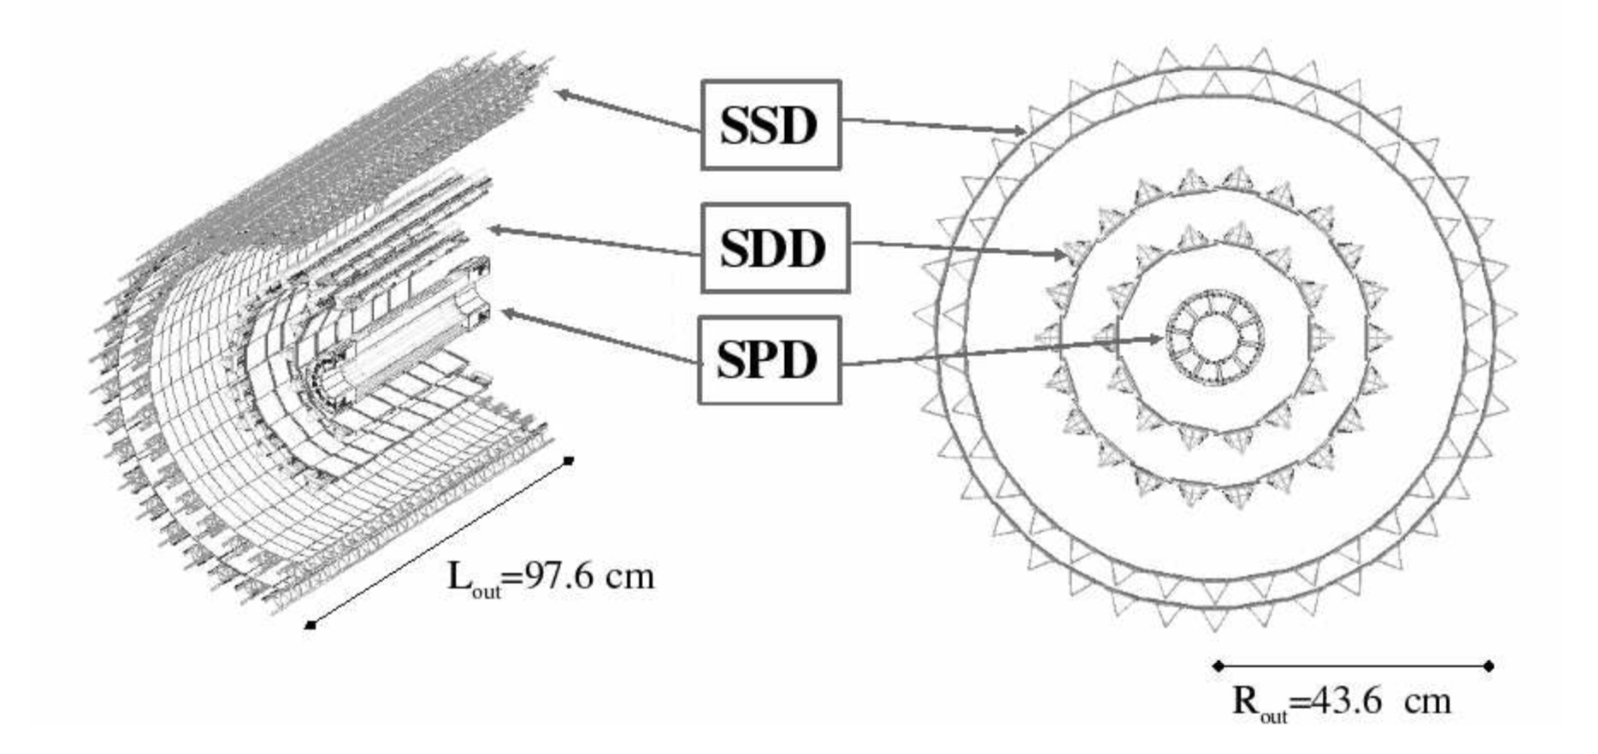
\includegraphics[width=0.95\textwidth]{pics/AliceITS}
\caption[ITS]{Schematic view of ALICE Inner Tracking System}
\label{fig:its}
\end{figure}


The main design guideline for the tracking detectors in ALICE was the requirement to have good track separation and high granularity in the high multiplicity environment of heavy ion collisions. Before the LHC started heavy ion runs the wildest estimates put the particle density at 8000 charged particles per unit of rapidity~\cite{ALICE}. In reality the particle density turned out to be significantly smaller, about 1600 charged particles per rapidity unit~\cite{Aamodt:2010pb}.

\setlength{\emergencystretch}{3em}

The main tracking detector in ALICE is the Time Projection Chamber (TPC)~\cite{Dellacasa:2000bm}. TPS is discussed in more detail in section ~\ref{sec:TPC}

Between TPC and the beam pipe there is an array of six layers of silicon detectors, called the inner tracking system (ITS)~\cite{Dellacasa:1999kf}. The main tasks of the ITS are to locate the primary vertex with a resolution better than \unit[100]{$\mu m$}, to reconstruct the secondary vertices from decaying particles, to track and identify particles with momenta below \unit[200]{$\mev$} and to compliment the momentum and angle measurements of TPC. During long shutdown 2 in 2019-2020 the entire ITS will be replaced~\cite{ITSupgrade}. As of 2018 the two innermost layers are made of the silicon pixel detector (SPD). As it is the closest detector to the interaction point it requires a very high spatial resolution. Thus the choice of pixel technology is natural. In heavy ion collisions the particle density is around 50 particles per $cm^2$. 

The next two layers together are the silicon drift detector (SDD). The layers are made out of homogeneous neutron transmutation doped silicon, that is ionized when a charged particle goes through the material. The generated charge then drifts to the collection anodes, where it is measured. The maximum drift time in SDD is about \unit[5]{$\mu s$}. This design gives very good multitrack capabilities and provides two out of the four $\nicefrac{dE}{dx}$ samples in the ITS.

The two remaining layers in the ITS are the silicon strip detector (SSD). The strips work in a similar way as silicon pixels, but by itself one layer only provides good resolution in one direction. Combining two crossing grids of strips provides 2 dimensional detection. Each charged particle will hit two intervening strips. The position of the hit can be deduced from the place where the strips cross each other.

\subsubsection{TPC}
\label{sec:TPC}
The time projection chamber (TPC) is a cylindrical detector filled with $ \unit[88]{m^3}$ of $\mathrm{Ne-CO_2}$ (90/10 \%) gas mixture. The gas is contained in a field cage that provides an uniform electric field of $\unit[400]{\nicefrac{V}{cm}}$ along the z-axis. Charged particles traversing through the TPC volume will ionise the gas along their path. This liberates electrons that drift towards the end plates of the cylinder. A schematic of the TPC is shown in Fig.~\ref{fig:tpc}.

The field cage is separated into two detection volumes by the central high voltage electrode. Both sides have a drift length of \unit[2.5]{m} and inner and outer diameters of \unit[1.2]{m} and \unit[5]{m} respectively. This means the central electrode must provide a maximum potential of \unit[100]{kV} to achieve the design field magnitude. The maximum time required for electrons to drift through the chamber is about \unit[90]{$\mu s$}.

When electrons reach the end of the main cylinder they enter the readout chambers. The readout section of both sides consists of 18 outer chambers and 18 inner chambers. Each of them is made of multiwire proportional chambers with cathode pad readouts. This design has been used in many TPCs before. During LS2 in 2019-2020, the multiwire chambers will be replaced by Gas Electron Multipliers (GEMs, see section \ref{sec:tpcupgrade}).

%The relatively slow drift time of 90 $\mu s$ is the limiting factor for the luminosity ALICE can take. The occupancy of the TPC must be kept in a manageable level. 


\subsubsection{TPC upgrade}
\label{sec:tpcupgrade}
\begin{figure}[htb]
\centering
\includegraphics[width=0.95\textwidth]{pics/alice-tpc-schematic}
\caption[TPC]{Schematic view of ALICE Time Projection Chamber}
\label{fig:tpc}
\end{figure}

During LS2 in 2019-2020 ALICE will go through significant modifications. The goal is to be able have continuous readout ~\cite{aliceupgrade} in heavy ion collisions at an interaction rate of 50 kHz. 
ALICE will add a new Forward Interaction trigger (FIT) to replace the V0 and T0 detectors. 

Additionally the current inner tracking system (ITS) will be completely replaced. The current layered structure with three different technologies will be replaced by an all pixel detector with significantly reduced pixel size. Additionally the first layer will be brought closer to the beam pipe. The new ITS will have better tracking efficiency and better impact parameter resolution. 

\setlength{\emergencystretch}{3em}

The muon detection will be complimented by the Muon Forward Tracker (MFT)~\cite{CERN-LHCC-2015-001}. Based on the same technology as the new ITS, MFT will be placed before the hadron absorber that sits in front of the existing muon spectrometer. MFT should significantly increase the signal/background ratio in heavy quark measurements.

Many subdetectors will make small improvements to enhance the readout rate. The central trigger processor will be replaced and ALICE will introduce a new framework $O^2$ that combines both online data acquisition and offline analysis.

The detector restricting the readout the most at the moment is the TPC. The current wire chamber based system  limits the readout rate to 3.5 kHz. To achieve the 50 kHz readout rate goal the wire chambers will be replaced by a Gas Electron Multiplier (GEM) based system. The GEMs are designed to minimise ion backflow to allow continuous, ungated and untriggered readout. I have made a personal contribution to the quality assurance of the new GEM readout of TPC.

TPC has a total of 36 inner and 36 outer readout chambers. Each of these will consist of 4 layers of GEM foils. The inner chambers will only have one foil for each layer. The outer chambers are separated into three sections, each with its own layer of foils. Each GEM foil is made up of a 50 $\mathrm{\mu m}$ thick resistive capton layer, coated on both sides by $5 \mathrm{\mu m}$ thick layers of copper. Each foils is separated into a number (20-24 depending on the size of the foil) of distinct active areas. The active areas are pierced densely with holes. They have 50-100 holes in the area of a single $\mathrm{mm^2}$. The density of holes changes from layer to layer. The two middle layers of foils have a larger (double) pitch (smaller hole density) while the top and bottom layers have a smaller (normal) pitch (larger hole density).

The purpose of the multilayered structure is to reduce the ion backflow~\cite{missing}; not only one layer of GEM foils will be installed, but a 4 layer stack. In the stack there are 2 standard pitch GEM foils, where the pitch size, i.e. the separation of the holes inside a foil is around 140 $\mu m$, and 2 large pitch GEM foils, there the hole spacing is two times larger, 280 $\mu m$. The two outer layers will have standard pitch and the two middle layers have large pitch. The middle layers with large pitch serve as extra insulator against the ion backflow. Additionally the setup allows operating individual GEM foils at lower voltages and still have an increase in the gain of a few orders of magnitude. ~\cite{TPCupgrade}

The holes have a conical shape which they acquire during a two step chemical etching process. The designed inner and outer diameters of the holes are $50\pm5 \mathrm{\mu m}$ and $70 \pm 5 \mathrm{\mu m}$ respectively. Fig.~\ref{fig:gem} shows the cross-section of a hole alongside with the operation principle of a GEM foil.

\begin{figure}[htb]
\centering
\documentclass[border=5mm]{standalone}
\usepackage{tikz}
\usetikzlibrary{positioning}
\usetikzlibrary{intersections, calc, fadings}
\usetikzlibrary{shadows.blur}

\usetikzlibrary{decorations.pathmorphing}
\usetikzlibrary{decorations.markings}
\begin{document}
\definecolor{primary}{HTML}{0000FF}
\definecolor{secondary}{HTML}{FF8000}
\definecolor{tertiary}{HTML}{00FFFF}
\tikzset{
photon/.style={decorate, decoration={snake}, draw=red},
particlearrow/.style={draw=blue, postaction={decorate},
    decoration={markings,mark=at position .5 with {\arrow[draw=black]{>}}}},
antiparticlearrow/.style={draw=blue, postaction={decorate},
    decoration={markings,mark=at position .5 with {\arrow[draw=black]{>}}}},
particle/.style={draw=blue},
antiparticle/.style={draw=blue},
gluon/.style={decorate, draw=orange,
    decoration={coil,amplitude=4pt, segment length=5pt}}
 }

\begin{tikzpicture}[scale=0.75]
\def\cone{(0,0)  -- (1,1) -- (0,2) -- (3,2) -- (2,1) -- (3,0) -- (0,0)}
%\draw[blue]\cone ;
\draw[draw=none,blur shadow = {shadow blur steps=5}] (-2,0) rectangle (10,2);
\shade[bottom color = black!50, top color =black!10] (-2,0) rectangle (10,1);
\shade[bottom color = black!20, top color =black!50] (-2,1) rectangle (10,2);

%\draw[blue, thick, postaction={decorate},
%    decoration={markings,mark=at position .25 with {\arrow[draw=blue]{>}}}] plot [smooth cycle, tension=0.6] coordinates {(5,1) (5.2,2.5) (5.8,2.5) (6,2) (6,0) (5.8,-0.5) (5.2,-0.5)};
\begin{scope}
\clip (4.6,-2) rectangle (8.9,4);
\draw[blue,postaction={decorate}, decoration={markings,mark=at position 0.25 with {\arrow[draw=blue]{>}}}] (5.6,1) ellipse (0.5cm and 1cm);
\draw[blue,postaction={decorate}, decoration={markings,mark=at position 0.25 with {\arrow[draw=blue]{>}}}] (5.55,1) ellipse (0.7cm and 1.5cm);
\draw[blue,postaction={decorate}, decoration={markings,mark=at position 0.25 with {\arrow[draw=blue]{>}}}] (5.5,1) ellipse (0.9cm and 2.5cm);
\draw[blue,postaction={decorate}, decoration={markings,mark=at position 0.125 with {\arrow[draw=blue]{>}}}] (5.45,1) ellipse (1.1cm and 5.5cm);

\draw[blue,postaction={decorate}, decoration={markings,mark=at position 0.375 with {\arrow[draw=blue]{<}}}] (8.05,1) ellipse (1.1cm and 5.5cm);
\draw[blue,postaction={decorate}, decoration={markings,mark=at position 0.25 with {\arrow[draw=blue]{<}}}] (7.9,1) ellipse (0.5cm and 1cm);
\draw[blue,postaction={decorate}, decoration={markings,mark=at position 0.25 with {\arrow[draw=blue]{<}}}] (7.95,1) ellipse (0.7cm and 1.5cm);
\draw[blue,postaction={decorate}, decoration={markings,mark=at position 0.25 with {\arrow[draw=blue]{<}}}] (8.0,1) ellipse (0.9cm and 2.5cm);
\draw[blue,postaction={decorate}, decoration={markings,mark=at position 0.95 with {\arrow[draw=blue]{>}}}] (6.75,-2) -- node[pos=0.05,fill=white] () {$\vec E$} (6.75,4);





\end{scope}

\begin{scope}
%\clip\cone ;
\clip (-2,0) -- (0,0) -- (0.5,1) -- (0,2) -- (-2,2);
\shade[top color = orange, bottom color=orange!70] (-2,0) rectangle (5,2);
\fill[black] (-2,0.2) rectangle (5,1.8);%\clip (C1) circle (2cm);
%\fill[secondary] (C2) circle (2cm);
\end{scope}
\begin{scope}
\clip (2.5,2) -- (5.5,2) --  (6,1) -- (5.5,0) -- (2.5,0) -- (2,1) -- (2.5,2);
\shade[top color = orange, bottom color=orange!70] (-2,0) rectangle (10,2);
\fill[black] (-2,0.2) rectangle (10,1.8);
\end{scope}

\begin{scope}
\clip (10,0) -- (8,0) -- (7.5,1) -- (8,2) -- (10,2);
\shade[top color = orange, bottom color=orange!70] (7.5,0) rectangle (10,2);
\fill[black] (7.5,0.2) rectangle (10,1.8);
\end{scope}

\draw[dashed] (0,2) -- (0,3.5);
\draw[dashed] (2.5,2) -- (2.5,3.5);
\draw[dashed] (0.5,1) -- (0.5,2.5);
\draw[dashed] (2,1) -- (2,2.5);
\draw[<->] (0,3.5) -- node[midway,fill=white] {$d_\mathrm{out}$} (2.5,3.5);
\draw[<->] (0.5,2.5) -- node[midway, fill=white] {$d_\mathrm{in}$} (2,2.5);
\draw[<->] (2.5,-1) -- node[midway,fill=white] {Pitch} (5.5,-1);
\draw[dashed] (2.5,0) -- (2.5,-1);
\draw[dashed] (5.5,0) -- (5.5,-1);

%Zoom box
\draw[thick, color=black!90] (6.5,0.75) rectangle (7,1.25);
\draw[thin,dashed,color=black!90] (6.5,0.75) -- (10.5,-2.5);
\draw[thin,dashed,color=black!90] (6.5,1.25) -- (10.5,6);
\draw[color=black!90] (10.5,-2.5) rectangle (17,6);


\tikzstyle{atom} = [circle,fill=orange, draw=orange, text centered, radius=1em, blur shadow = {shadow blur steps=5} ] 


\draw[thin, gray, ->] (11,-2) -- node[midway] (E) {}(11,5);
\draw[thin, gray, ->] (12,-2) -- (12,5);
\draw[thin, gray, ->] (13,-2) -- (13,5);
\draw[thin, gray, ->] (14,-2) -- (14,5);
\draw[thin, gray, ->] (15,-2) -- (15,5);
\draw[thin, gray, ->] (16,-2) -- node[midway,label=right:$\vec E$] (E2) {}(16,5);


\node[atom,above right=2cm and 2cm of E] (vert1) {};
\coordinate[above right=1cm and 0.2 cm of vert1,label=below right:$e$] (e1);
\node[atom,below left=1.5cm and 0.5cm of vert1] (vert21) {};
\node[atom,below right=1.5cm and 0.5cm of vert1] (vert22) {};
\node[atom,below left=1.5cm and 0.2cm of vert21] (vert31) {};
\node[atom,below right=1.5cm and 0.2cm of vert21] (vert32) {};
\node[atom,below left=1.5cm and 0.2cm of vert22] (vert33) {};
\node[atom,below right=1.5cm and 0.2cm of vert22] (vert34) {};

\node[atom, right=1cm  of vert1] (a1) {};
\node[atom, left=1cm  of vert1,label=above:Atoms] (a2) {};
\node[atom, left=1cm  of vert21] (a3) {};
%\node[atom, right=1cm  of vert22] (a4) {};
%\node[atom, right=0.5cm  of vert34] (a5) {};
\node[atom, left=0.5cm  of vert31] (a6) {};



\coordinate[below left=1.5cm and 0.5 cm of vert31] (e2);
\coordinate[below right=1.5cm and 0.5 cm of vert31] (e3);
\coordinate[below left=1.5cm and 0.5 cm of vert32] (e4);
\coordinate[below right=1.5cm and 0.5 cm of vert32] (e5);
\coordinate[below left=1.5cm and 0.5 cm of vert33] (e6);
\coordinate[below right=1.5cm and 0.5 cm of vert33] (e7);
\coordinate[below left=1.5cm and 0.5 cm of vert34] (e8);
\coordinate[below right=1.5cm and 0.5 cm of vert34,label=above left:$e$] (e9);




\draw[particlearrow] (e1) to[out=225,in=90]  (vert1);
\draw[particlearrow] (vert1) to[out=225,in=90]  (vert21);
\draw[particlearrow] (vert1) to[out=-45,in=90]  (vert22);

\draw[particlearrow] (vert21) to[out=235,in=90]  (vert31);
\draw[particlearrow] (vert21) to[out=-55,in=90]  (vert32);
\draw[particlearrow] (vert22) to[out=235,in=90]  (vert33);
\draw[particlearrow] (vert22) to[out=-55,in=90]  (vert34);

\draw[particlearrow] (vert31) to[out=235,in=90]  (e2);
\draw[particlearrow] (vert31) to[out=-55,in=90]  (e3);
\draw[particlearrow] (vert32) to[out=235,in=90]  (e4);
\draw[particlearrow] (vert32) to[out=-55,in=90]  (e5);
\draw[particlearrow] (vert33) to[out=235,in=90]  (e6);
\draw[particlearrow] (vert33) to[out=-55,in=90]  (e7);
\draw[particlearrow] (vert34) to[out=235,in=90]  (e8);
\draw[particlearrow] (vert34) to[out=-55,in=90]  (e9);


\end{tikzpicture}
\end{document}
\caption{{\it left} Cross-section of a GEM foil. (Not to scale). The hole diameters are $d_\mathrm{in} = 50\pm5 \mathrm{\mu m}$ and $d_\mathrm{out} =70 \pm 5 \mathrm{\mu m}$ and pitch is either 140 or 280 $\mathrm{\mu m}$. {\it right} The amplification of a GEM foil is based on the Townsend avalanche phenomenon. Electrons entering the electric field inside the hole are accelerated. If they gain enough energy before colliding with atoms they can liberate additional electrons, which are further accelerated leading to a chain reaction.}
\label{fig:gem}
\end{figure}

The working principle of these foils is based on the Townsend avalanche phenomenon, which is also used in proportional counters such as Geiger counters. There is a large potential difference (140-400 V) applied to the two sides of the foil, which results in large field in each hole. Electrons gain energy in the field and if the electric field is strong enough, the free electron can gain sufficient velocity (energy) to liberate another electron when it next collides with a molecule. The two free electrons then travel along the electric field and can gain sufficient energy from the electric field to cause further impact ionisations, and so on, leading to a chain reaction. Under the right conditions a single electron entering any hole will create an avalanche containing 100–1000 electrons; this is the gain of the GEM foil. 
%This acts both as a lens and an amplifier for the electrons. The amplification happens inside the holes where the field is the strongest. 

As opposed to wire chambers, which typically have one voltage setting, a GEM-based detector requires several independent voltage settings: there is a drift voltage which drives the electrons from the ionisation point to the GEM, an amplification voltage, and an extraction voltage that brings electrons from the GEM exit to the readout plane. In a multilayer system this is further complicated by the voltages between layers of foils.



\subsubsection*{Quality Assurance of the GEM foils}
The GEM foils are produced at CERN, where they will undergo a basic QA (QA-B) procedure, that includes a coarse optical inspection for any large defects ($ \gtrsim \unit[1]{mm}$) and a short term high voltage measurement. Afterwards the foils are sent for an advanced quality assurance (QA-A) procedure which is performed in one of the two QA-A centers, one in the Helsinki Institute of Physics (HIP) and one in the Wigner Research Centre in Budapest. Details of the QA-A procedure can be found in the thesis of Márton Vargyas~\cite{MartonThesis} and in \cite{Brucken:2018rej}. In the QA-A centers all foils are put through a detailed optical scanning process and a long term high voltage measurement. I was personally performing the QA production in Helsinki for the final 6 months of the project.

The optical scan is performed with the help of a scanning robot. The setup along with most of the software was developed at the Detector Laboratory of the Helsinki Institute of Physics~\cite{Hilden:2014rba}. The optical scan is able to distinguish every single hole on the GEM foil and measure their properties. The purpose of the scan is two-fold; to catch defects that could affect the performance and classify the foils based on their hole parameters. It is expected that these are connected with the foil's electric properties~\cite{Hilden:2014rba}. For example, smaller holes create more intense and focused fields, which would result in larger amplification of their avalanche electrons, i.e. the local gain is expected to be larger.

After the optical scanning, the foils are subjected to a long term ( 5-12 hours) high voltage leakage current measurement. Each segment of the GEM foil is connected to a high voltage of $\unit[500]{V}$ and the leakage current is measured separately for each segment. The accepted leakage current in each segment is \unit[0.16]{nA}.

Foils that fail the criteria are either trashed or sent to CERN for recleaning or repairing, after which they will go through the QA pipeline again.

Additionally some foils will be put through a gain mapping procedure. As it is time consuming can only be performed in the QA-A center in Budapest it is only a small subset of foils. However, by measuring the gain in some foils the gain can be correlated with foil properties. Thus the single foil gain can be predicted based on the results of the optical scan. Details can be found in~\cite{MartonThesis}.


\subsubsection{Particle identification}
One guiding principle in the design of ALICE was to achieve good particle identification (PID) over  a large part of phases space and for several different particle types. In ALICE there are several detectors taking part in the identification of particles. 

One of the particle identification detectors is the transition radiation detector (TRD)~\cite{Cortese:519145}. Its main task is identifying electors with momenta larger than \unit[1]{\gev}. Transition radiation is produced when highly relativistic particles traverse the boundary between two media having different dielectric constants. The average energy of the emitted photon is approximately proportional to the Lorentz factor $\gamma$ of the particle, which provides an excellent way of discriminating between electrons and pion. ALICE TRD is made of a composite layer of foam and fibres. The emitted photons are then measured in six layers of Xe/CO2 filled time expansion wire chambers. 

The time of flight  (TOF) detector~\cite{Dellacasa:2000kh} uses a very simple physics principle, i.e. calculating the velocity of the particle using the time of flight between two points. Combining this with the momentum of particle, obtained from the tracking detectors, one can calculate the mass of the particle, which identifies particles. The TOF detector consists of multigap resistive wire chambers. These are stacks of resistive plates spaced equally. They allow time of flight measurements in large acceptance with high efficiency and with a resolution better than 100 ps. 

The third specific particle identification detector is the high momentum particle identification (HMPID) detector~\cite{Beole:1998yq}. The HMPID uses a ring imaging Cherenkov counter to identify particles with momenta larger than \unit[1]{\gev}. Particles moving through a material faster than the speed of light in the material will produce Cherenkov radiation. The velocity of the particle determines the angle at which the radiation is emitted. Measuring this angle gives the velocity of the particle. This can be again used to calculate the mass of the particle, if the momentum is known. In HMPID the material is a liquid radiator and the photons are measured with multiwire proportional chambers in conjunction with photocathodes. 

In addition to the specific particle identification detectors, the general purpose tracking detectors can be used for identification through the use of specific energy loss of charged particles traversing through a medium and the transition radiation emitted by charged particles when crossing the boundary between two materials. 

$\nicefrac{\mathrm{d}E}{\mathrm{d}x}$ measurements are provided by the last four layers of the ITS detector, i.e. the SDD and the SSD, thanks to their analog readout~\cite{ALICEpid}. ITS can provide particle identification in the low $\pt{}$ region, up to $~ \unit[1]{\gev}$, and pions reconstructed in the standalone mode can be identified down to $~100 \mev$. Similar to ITS the TPC detector provides specific energy loss measurements. TPC can identify charged hadrons up to $\pt{} ~ \unit[1-2]{\gev}$ as well as light nuclei, He3 and He4.


\subsubsection{Electromagnetic Calorimeter}
\label{sec:emcal}
Calorimeters are designed to measure the energy of particles. Electromagnetic calorimeters specialise in detecting particles that interact primarily through the electromagnetic interaction, namely photons and electrons. They are required in many neutral meson and direct photon analyses. In addition the energy information enhance jet measurements.
\setlength{\emergencystretch}{3em}


ALICE has two electromagnetic calorimeters, the photon spectrometer (PHOS)~\cite{PHOS} and the electromagnetic calorimeter (EMCal)~\cite{Cortese:2008zza}. PHOS is a homogeneous calorimeter that consists of scintillating $\mathrm{PbWO_4}$ crystals, which generate a bremsstrahlung  shower and produce scintillation light. The energy of the particle determines the amount of light produced. To improve the charged particle rejection, PHOS includes a charged particle veto detector (CPV)~\cite{cpv}. PHOS is built to have a very fine granularity, making it well suited for measuring direct photons and neutral mesons.

In comparison to PHOS, EMCal has coarser granularity, but a significantly larger acceptance, making it suitable for jet physics. The acceptance of EMCal in the azimuthal angle is $ 80\deg < \phi < 187 \deg$. During long shutdown 1 in 2013-2015, EMCal was extended with the di-jet calorimeter (DCal) ~\cite{DCAL}, giving an additional acceptance region of $ 260\deg < \phi < 320 \deg$. This provides partial back-to-back coverage. 

EMcal is segmented into 10 full size super modules (SM), 5 for A side and 5 for C side, and two 1/3 sized SMs, one for each side. This segmentation can be seen in Fig.~\ref{fig:emcal}. Each SM is divided into 24 strips, each covering full $\eta$ (24 towers) and 2 towers in $\eta$. Each strip is composed of $2\times2$ tower modules. Thus each full size super module includes 1152 towers and in total the EMCal is made up of 12288 towers.

\begin{figure}[htb]
\centering
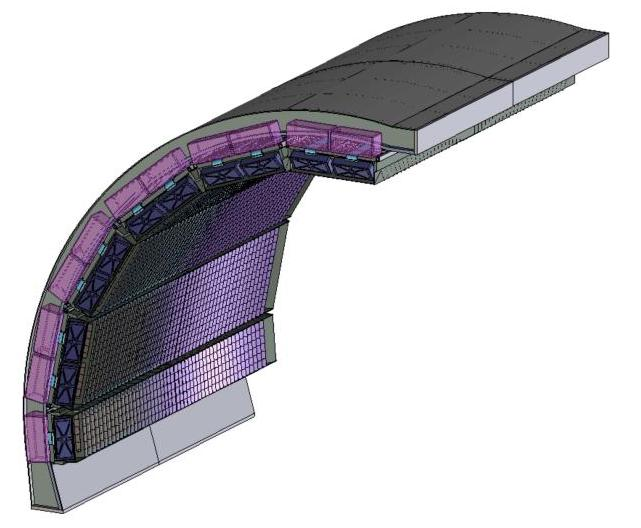
\includegraphics[width=0.9\textwidth]{figures/fullemcal}
\caption{The EMCal detector arc, where the segmentation into 10 full size and 2 $\nicefrac{1}{3}$-sized (5 and 1 per side) supermodules can be seen.}
\label{fig:emcal}
\end{figure}

The build of individual towers is shown in Fig.~\ref{fig:emcaltower}. Each tower is built up from 76 alternating layers of 1.44 \unit{mm} Pb and 77 layers of 1.76 \unit{mm} polystyrene base injection moulded scintillator. The lead tiles produce the shower and scintillator tiles the light. Each tower scintillator is equipped with reflectors on all sides to provide better gain and keep the four towers inside one module isolated. The scintillation photons produced in the active volume of the tower are collected by 36 longitudinally placed wave length shifting light guide fibres. The light is eventually directed to the Avalanche Photo Diodes (APD) for readout. 

\begin{figure}[htb]
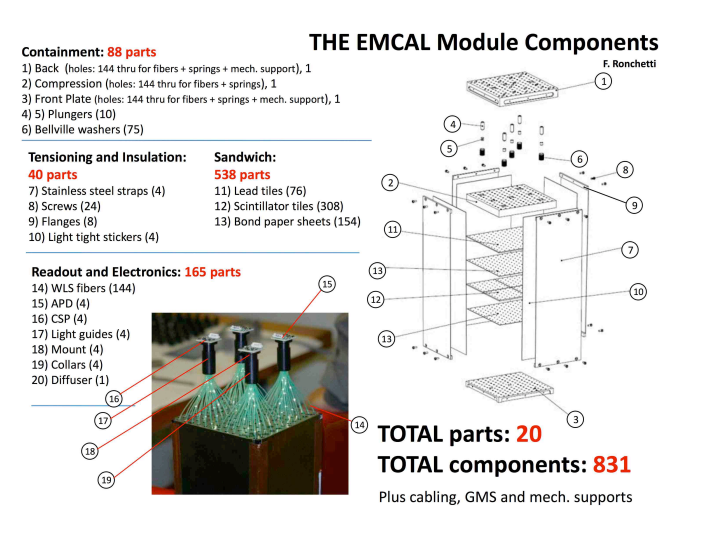
\includegraphics[width=0.9\textwidth]{pics/EMCAL_components}
\caption{The exploded EMCal tower view}
\label{fig:emcaltower}
\end{figure}


\subsubsection{Forward and trigger detectors}
\label{sec:forward}
ALICE includes a few small and specialised detectors of importance. The event time is determined with very good precision (< 25 ns) by the T0 detector~\cite{Cortese:2004aa}. T0 consists of two sets of Cherenkov counters that are mounted around the beam pipe on both sides of the interaction point. T0 gives the luminosity measurement in ALICE.

Another small detector in the forward direction is the V0 detector~\cite{Cortese:2004aa}. This consists of two arrays of segmented scintillator counters located at $-3.7 < \eta < -1.7$ and $ 2.8 < \eta < 5.1$. V0 is used as a minimum bias trigger and for rejection of beam-gas background. Particle multiplicity in the forward direction can be related to the event centrality. Thus V0 is the main detector used in centrality determination in PbPb collisions.

The multiplicity measurement of V0 is complimented by the forward multiplicity detector (FMD)~\cite{Cortese:2004aa}. FMD includes five rings of silicon strip detectors that make up the FMD. FMD gives acceptance in the range $-3.4 < \eta < -1.7$ and $ 1.7 < \eta < 5.0$.

During long shutdown 2 in 2019-2020, V0 and T0 will be replaced by the Fast Interaction Trigger (FIT) detector~\cite{Maevskaya:2018ggm}. For historical reasons elements of FIT are also referred to as V0+ and T0+. FIT will allow centrality, event plane, luminosity and interaction time determination in the continuous readout mode, that ALICE will operate in after 2020.

For photon multiplicity measurement ALICE has the photon multiplicity detector (PMD) ~\cite{CERN-LHCC-99-032}. PMD uses two planes of gas proportional counters with a cellular honeycomb structure. PMD gives the multiplicity and spatial distribution of photons in the region $2.3 < \eta < 3.7$.

On top of the ALICE magnet there is an array of 60 large scintillators called the ALICE cosmic ray detector (ACORDE) ~\cite{Fernandez:2006ki}. ACORDE is used as a trigger for cosmic rays for calibration and alignment. 

The only hadronic calorimeters in ALICE are the zero degree calorimeters (ZDC)~\cite{Dellacasa:1999ke}, which are located next to the beam pipe in the machine tunnel about 116 m from the interaction point. There are two sets of calorimeters. One is made of tungsten, specialising in measuring neutrons, while the other, made of brass, is specialised in measuring protons. ZDC is meant to detect spectators, i.e. parts of the colliding ions that do not take part in the interaction. If there are more spectators, the collisions is likely to be more peripheral. Thus ZDC gives information about the centrality of the event especially in proton-lead collisions~\cite{Adam:2014qja}, but also in~\PbPb collisions~\cite{Abelev:2013qoq}.

A new detector installed during the long shutdown 1 is the ALICE diffractive detector (AD)~\cite{AD}. AD consists of two assemblies, one in each side of the interaction point, both made of two layers of scintillators. These assemblies are situated about 17 m and 19.5 m away from the interaction points. The pseudorapidity coverage is $-6.96 < \eta < -4.92 $ and $4.78 < \eta < 6.31$. AD greatly enhances ALICE's capability for diffractive physics measurements that require a large pseudorapidity gap.

\subsubsection{Muon spectrometer}
Outside the main magnet, ALICE has a spectrometer dedicated to measuring muons~\cite{Beole:1996yp}. In heavy ion physics muons are mainly used to measure the production of the heavy quark resonances $\nicefrac{J}{\psi}, \Psi^{'}, \Upsilon, \Upsilon^{'}$ and $\Upsilon^{''}$.

The muon spectrometer consists of three parts, the absorber, the muon tracker and the muon trigger. The absorber is meant to remove the hadronic background as efficiently as possible. After the absorber there are ten plates of thin cathode strip tracking stations with high granularity, the muon tracker. After the muon tracker there is a layer of iron to filter out any remaining particles, other than muons. The muon trigger is located behind this layer. The trigger consists of four resistive plate chambers. 

\subsubsection{Triggers}
\label{sec:trigger}
High energy physics experiments need triggers to select interesting physics. Experiments such as CMS and ATLAS at CERN look for extremely rare events with up to 40 million events each second. Such amounts can't be recorded real-time as many detectors require some time for the readout, up to 1 ms/event in ALICE. Thus one uses triggers, i.e. a set of very fast hardware based decisions on which events are to be saved. Additionally one needs some confirmation that an event has even occurred to tell other detectors that the event needs to be recorded. 

For ALICE the target event rates are \unit[1]{MHz} for \pp collisions, 0.1-2 \unit{kHz} for \PbPb collisions and 200 \unit{kHz} for the 2013 \pPb collisions.

At ALICE the main system responsible for the trigger decisions is the ALICE Central Trigger Processor (CTP)~\cite{ctp}. The CTP generates three levels of hierarchical hardware triggers - Level 0, Level 1 and Level 2, (L0, L1 and L2 respectively) before an event is accepted and transmitted to the Data Acquisition system (DAQ). Afterwards additional software assessments are performed by the High Level Trigger (HLT).

Triggers can be roughly put into two classes, minimum bias triggers that make sure no empty events are recorded, and rare triggers that require specific signatures in ALICE detectors, such as large energy deposits in EMCal or two muons in the muon arm acceptance.

\subsubsection*{Minimum bias trigger}
Several of the ALICE detectors are used to make the initial minimum bias trigger decisions. These include the SPD layers of ITS, V0 and T0. SPD can count the number of hits in the first two layers of ITS. Minimum bias \pp collisions typically require at least one hit in either SPD or V0A/V0C. Similarly \PbPb triggers look at both V0 and SPD hits. The \pPb data has been mainly triggered using V0 information.


\subsubsection*{EMCal trigger}
In addition to the minimum bias triggers, the most relevant trigger for this thesis is the EMCal trigger. Much of the EMCal trigger has been developed at the University of Jyväskylä. Extensive details of the trigger and the development work can be found in the thesis of Ji\v ri Král~\cite{JiriThesis}. Personally I have spent time at CERN helping in the maintenance of the level 0 trigger.

ALICE EMCal provides two levels of trigger signal, L0 and L1, which allows triggering on either single shower deposits or integrated energy deposits in larger ares, i.e. jets~\cite{KRAL2012261}.

As inputs the trigger gets exclusive sets of $2\times2$ EMCal towers, to limit the number of channels that need to be processed. The L0 trigger then checks for energy deposits within a rolling window of $2\times2$ trigger channels ($4\times4$ towers). Areas of $4\times4$ towers most probably will contain only a single shower. (or two adjacent showers coming from a single decayed $\pi^0$) Thus the trigger is called the single shower trigger. 

For L0 the trigger decision is done in Trigger Region Units (TRU) that each cover $4\times42$ channels ($8\times48$ towers). The amplitude from the sliding window is compared to a constant threshold. Additionally a peak finding algorithm is implemented to define correctly the time of the signal maximum. A single bit OR decision of all individual TRUs is forwarded to the CTP as the EMCal L0 trigger decision.

The L0 information is additionally forwarded to the Level 1 trigger, which recomputes similar $2\times2$ channel decisions to produce the single shower trigger, but L1 can perform the calculation also on the borders between trigger units. In addition the L1 trigger can  check for energy deposits inside a larger $16\times16$ channel ($32\times32$ towers) window, which is considered to be the jet trigger.

The L1 trigger can compare up to two thresholds for each single shower and jet trigger. There is a dedicated link in between the V0 detector and EMCal STU, which can provide centrality information that is used to compute a dynamical threshold as a function of the V0 multiplicity.

The trigger subsystem provides both the L0 and L1 decisions to the CTP and DAQ. 
%
%\begin{figure}
%\includegraphics[0.9\textwidth]{}
%\caption{Level 0 trigger rejection factor for clusters and jets}
%\end{figure}
